\documentclass{article}
\usepackage{graphicx} % Required for inserting images
\usepackage{float}
\usepackage{geometry}
\usepackage{hyperref}
\usepackage{listings}

% Set page margins
\geometry{
    a4paper,
    left=2.5cm,
    right=2.5cm,
    top=2.5cm,
    bottom=2.5cm,
}

% Hyperlink colors
\hypersetup{
    colorlinks=true,
    linkcolor=blue,
    filecolor=magenta,      
    urlcolor=cyan,
}

% Code listing style setup
\usepackage{xcolor}
\definecolor{codegreen}{rgb}{0,0.6,0}
\definecolor{codegray}{rgb}{0.5,0.5,0.5}
\definecolor{codepurple}{rgb}{0.58,0,0.82}
\definecolor{backcolour}{rgb}{0.95,0.95,0.92}

\lstdefinestyle{mystyle}{
    backgroundcolor=\color{backcolour},   
    commentstyle=\color{codegreen},
    keywordstyle=\color{magenta},
    numberstyle=\tiny\color{codegray},
    stringstyle=\color{codepurple},
    basicstyle=\ttfamily\footnotesize,
    breakatwhitespace=false,         
    breaklines=true,                 
    captionpos=b,                    
    keepspaces=true,                 
    numbers=left,                    
    numbersep=5pt,                  
    showspaces=false,                
    showstringspaces=false,
    showtabs=false,                  
    tabsize=2
}
\lstset{style=mystyle}

% Task
% Background
% In the above Manual module, we conducted related exercises utilizing the
% APOBEC3A mRNA sequences. In the Task module, we will analyze the APOBEC3A
% coding protein. APOBEC (apolipoprotein B mRNA editing catalytic polypeptide-
% like) proteins have a characteristic zinc-coordination motif (H-X-E-X23-28-P–C-X-
% C) within the active site where a water molecule binds Zn2+ and the metal ion is
% coordinated by one histidine and two cysteines. The AID/APOBEC family enzymes
% convert cytosines in single-stranded DNA to uracil causing base substitutions and
% strand breaks. Based on this property, relevant research has used human
% APOBEC3A (hAPOBEC3A) fusion dead Cas9 (dCas9) protein as a base editor for
% precise genome editing.

% Task1. Using the human APOBEC3A (hAPOBEC3A) protein sequence (ID: NP_663745.1)
% as query, use BLASTp to search for its homologous protein sequence.

% Task2. For the APOBEC3A.fasta file (from iSpace), perform multiple sequence alignment
% and construct phylogenetic tree.

% Task3. Attempt to interpret the results of this phylogenetic tree.

% Task4. Based on the phylogenetic tree, select the sequences closest to hAPOBEC3A
% and generate pairwise sequence alignment, attempt to interpret the specific
% differences between the two sequences (hAPOBEC3A and target sequence).

% Closest: Pongo pygmaeus APOBEC3A protein


\title{Bioinfo Lab 1}
\author{Bohan YANG}
\date{September 2025}

\begin{document}

\maketitle

\section{Task 1}

\begin{center}
    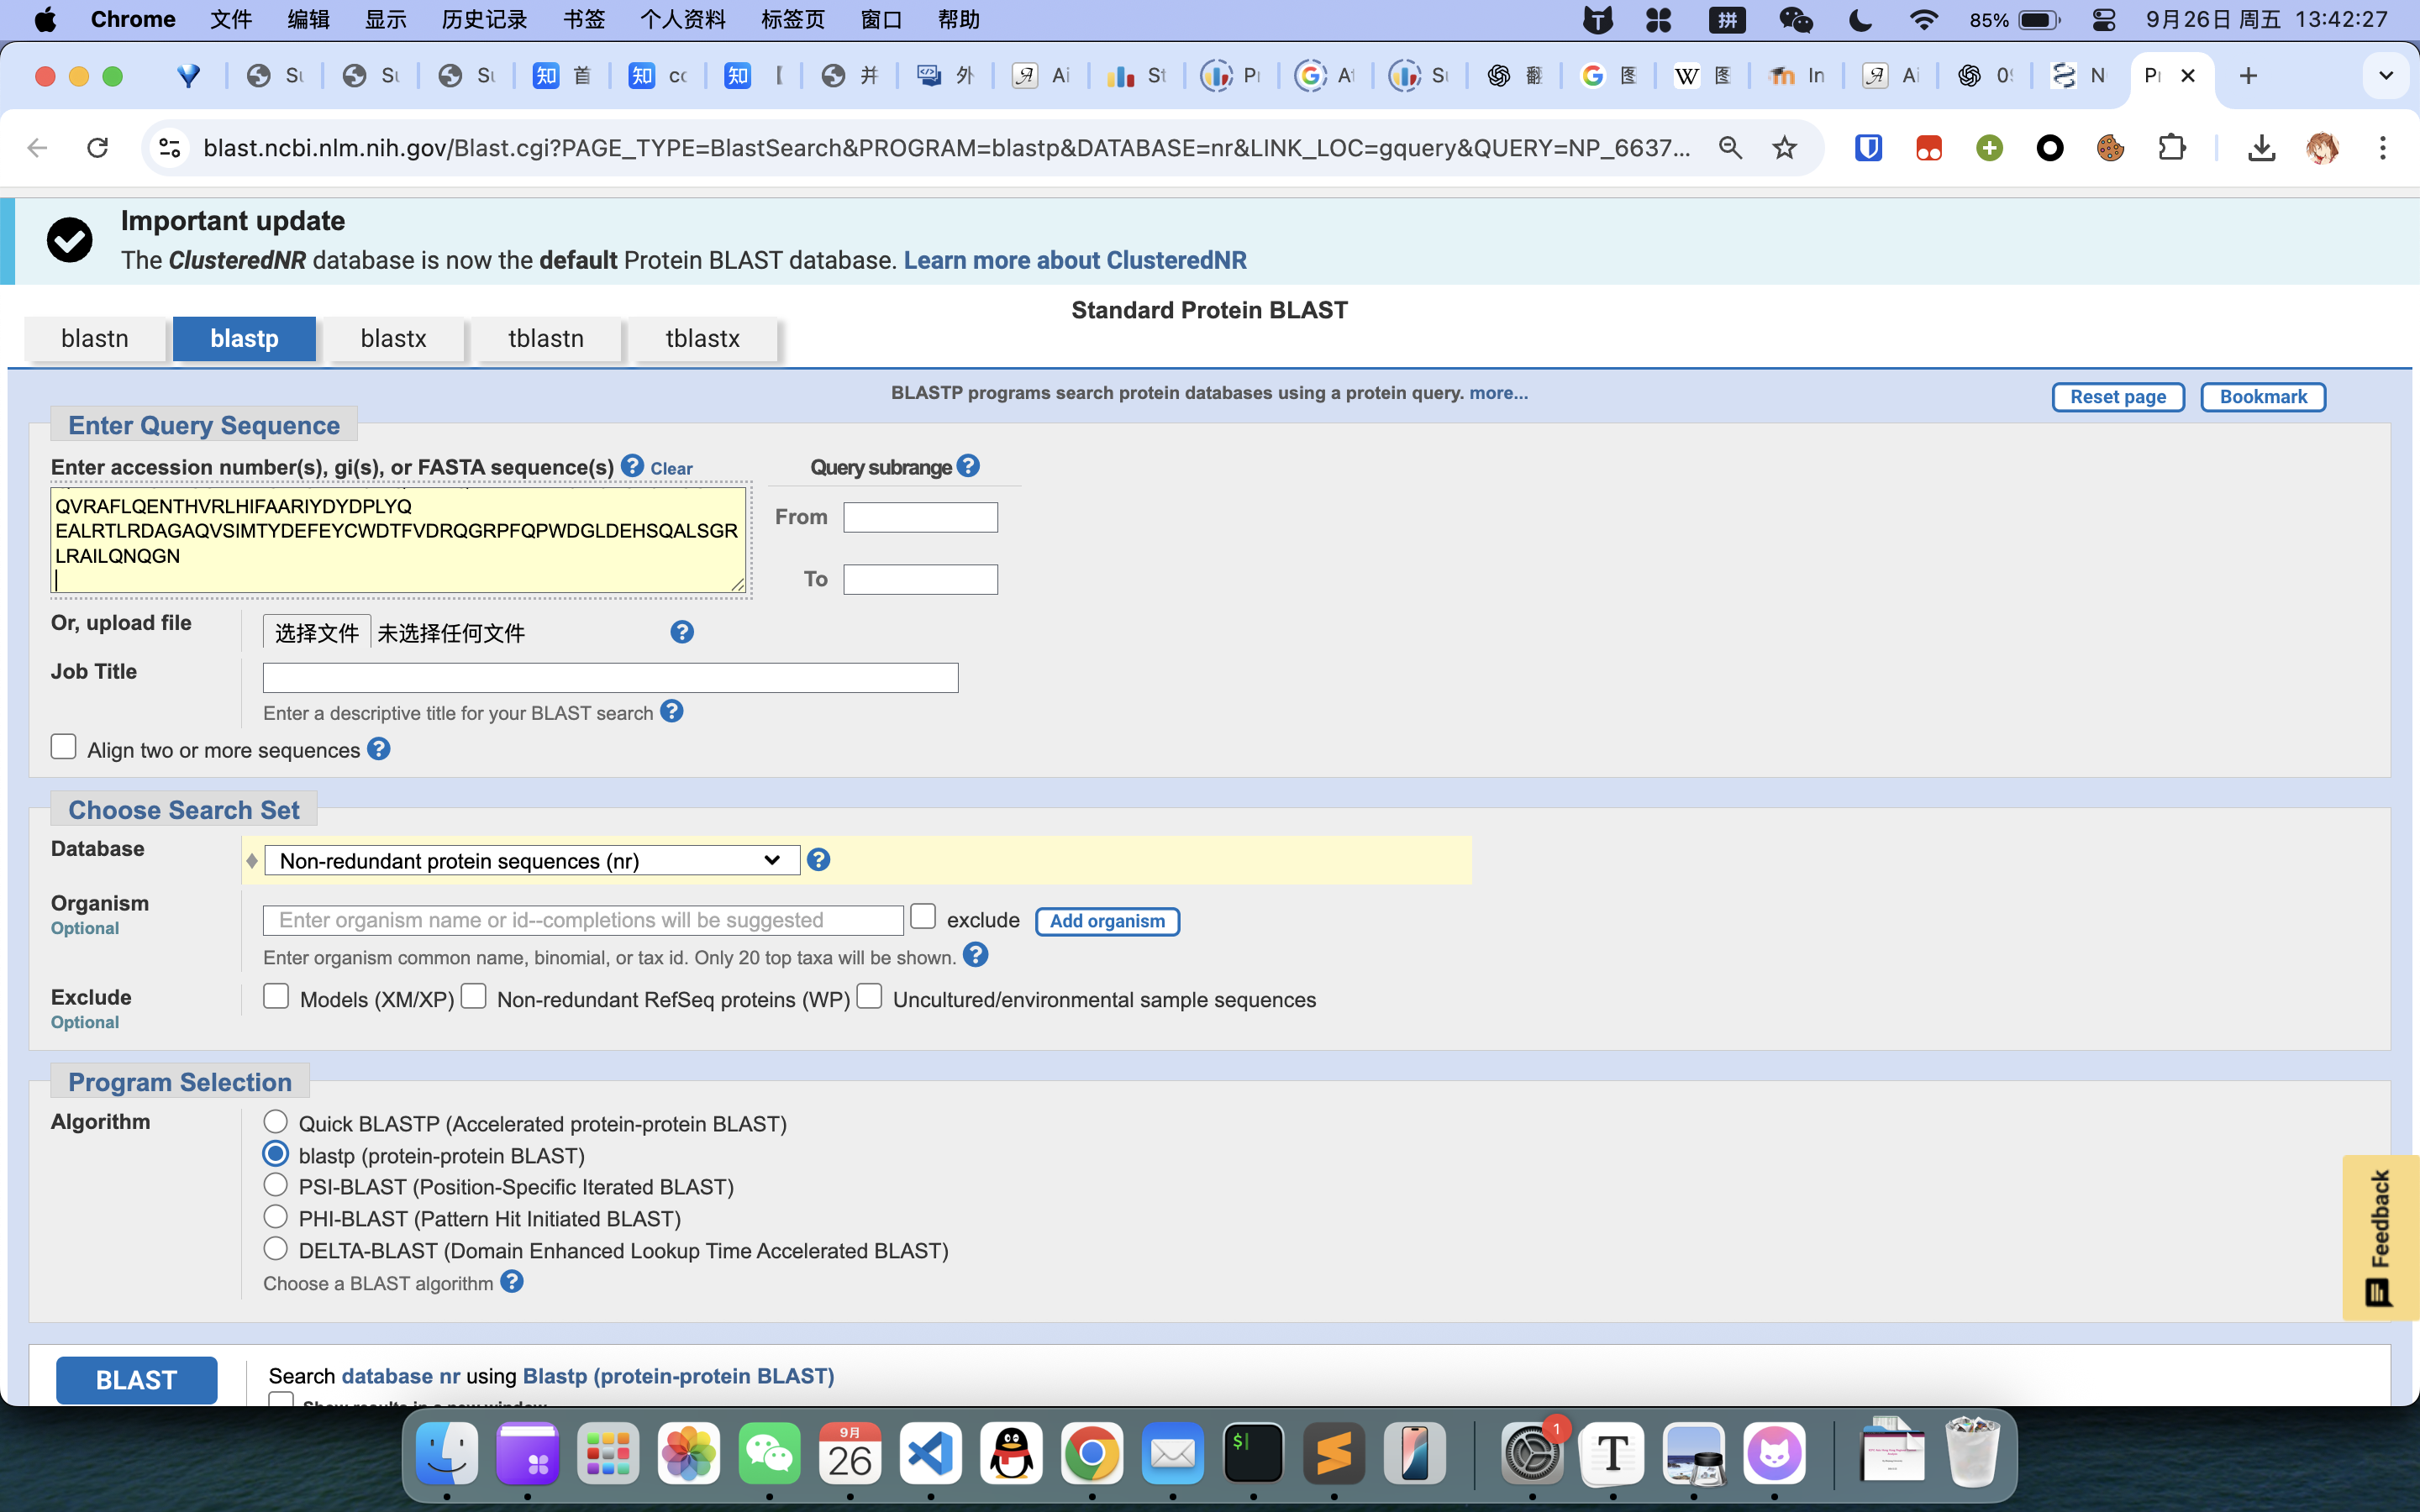
\includegraphics[width=1\textwidth]{../images/task1/image1.png}
\end{center}
\begin{center}
    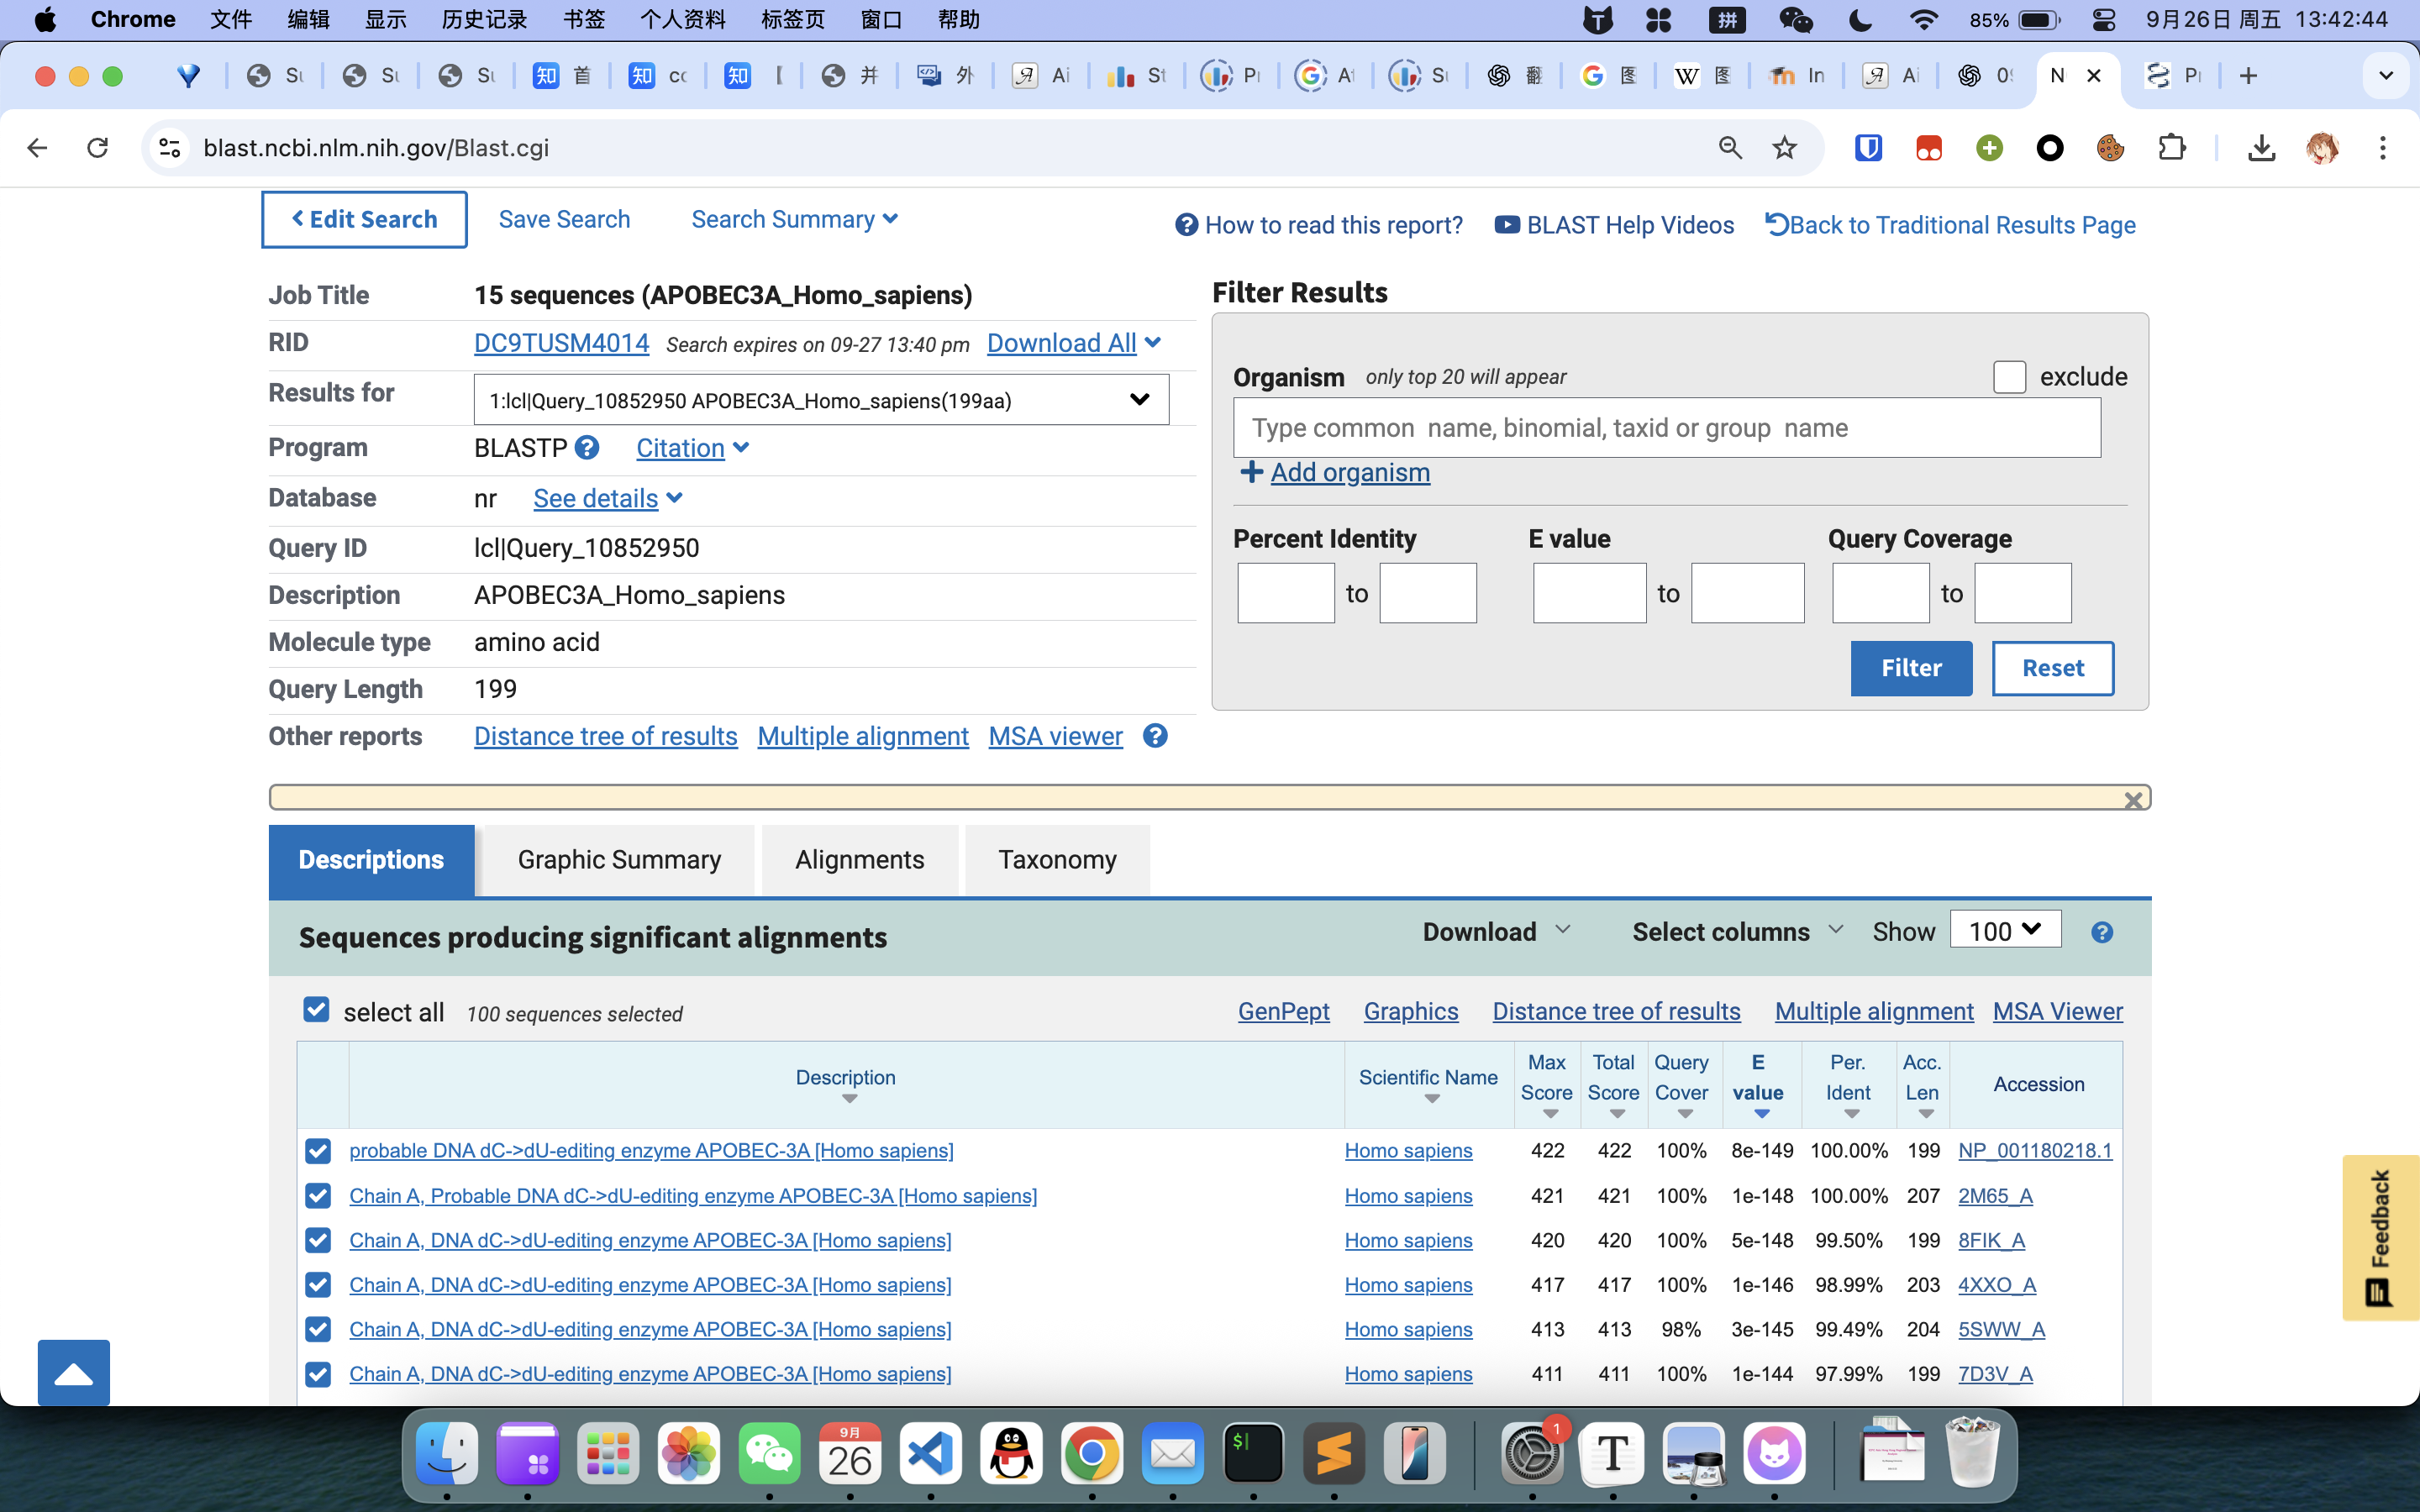
\includegraphics[width=1\textwidth]{../images/task1/image2.png}
\end{center}

\section{Task 2}

\begin{center}
    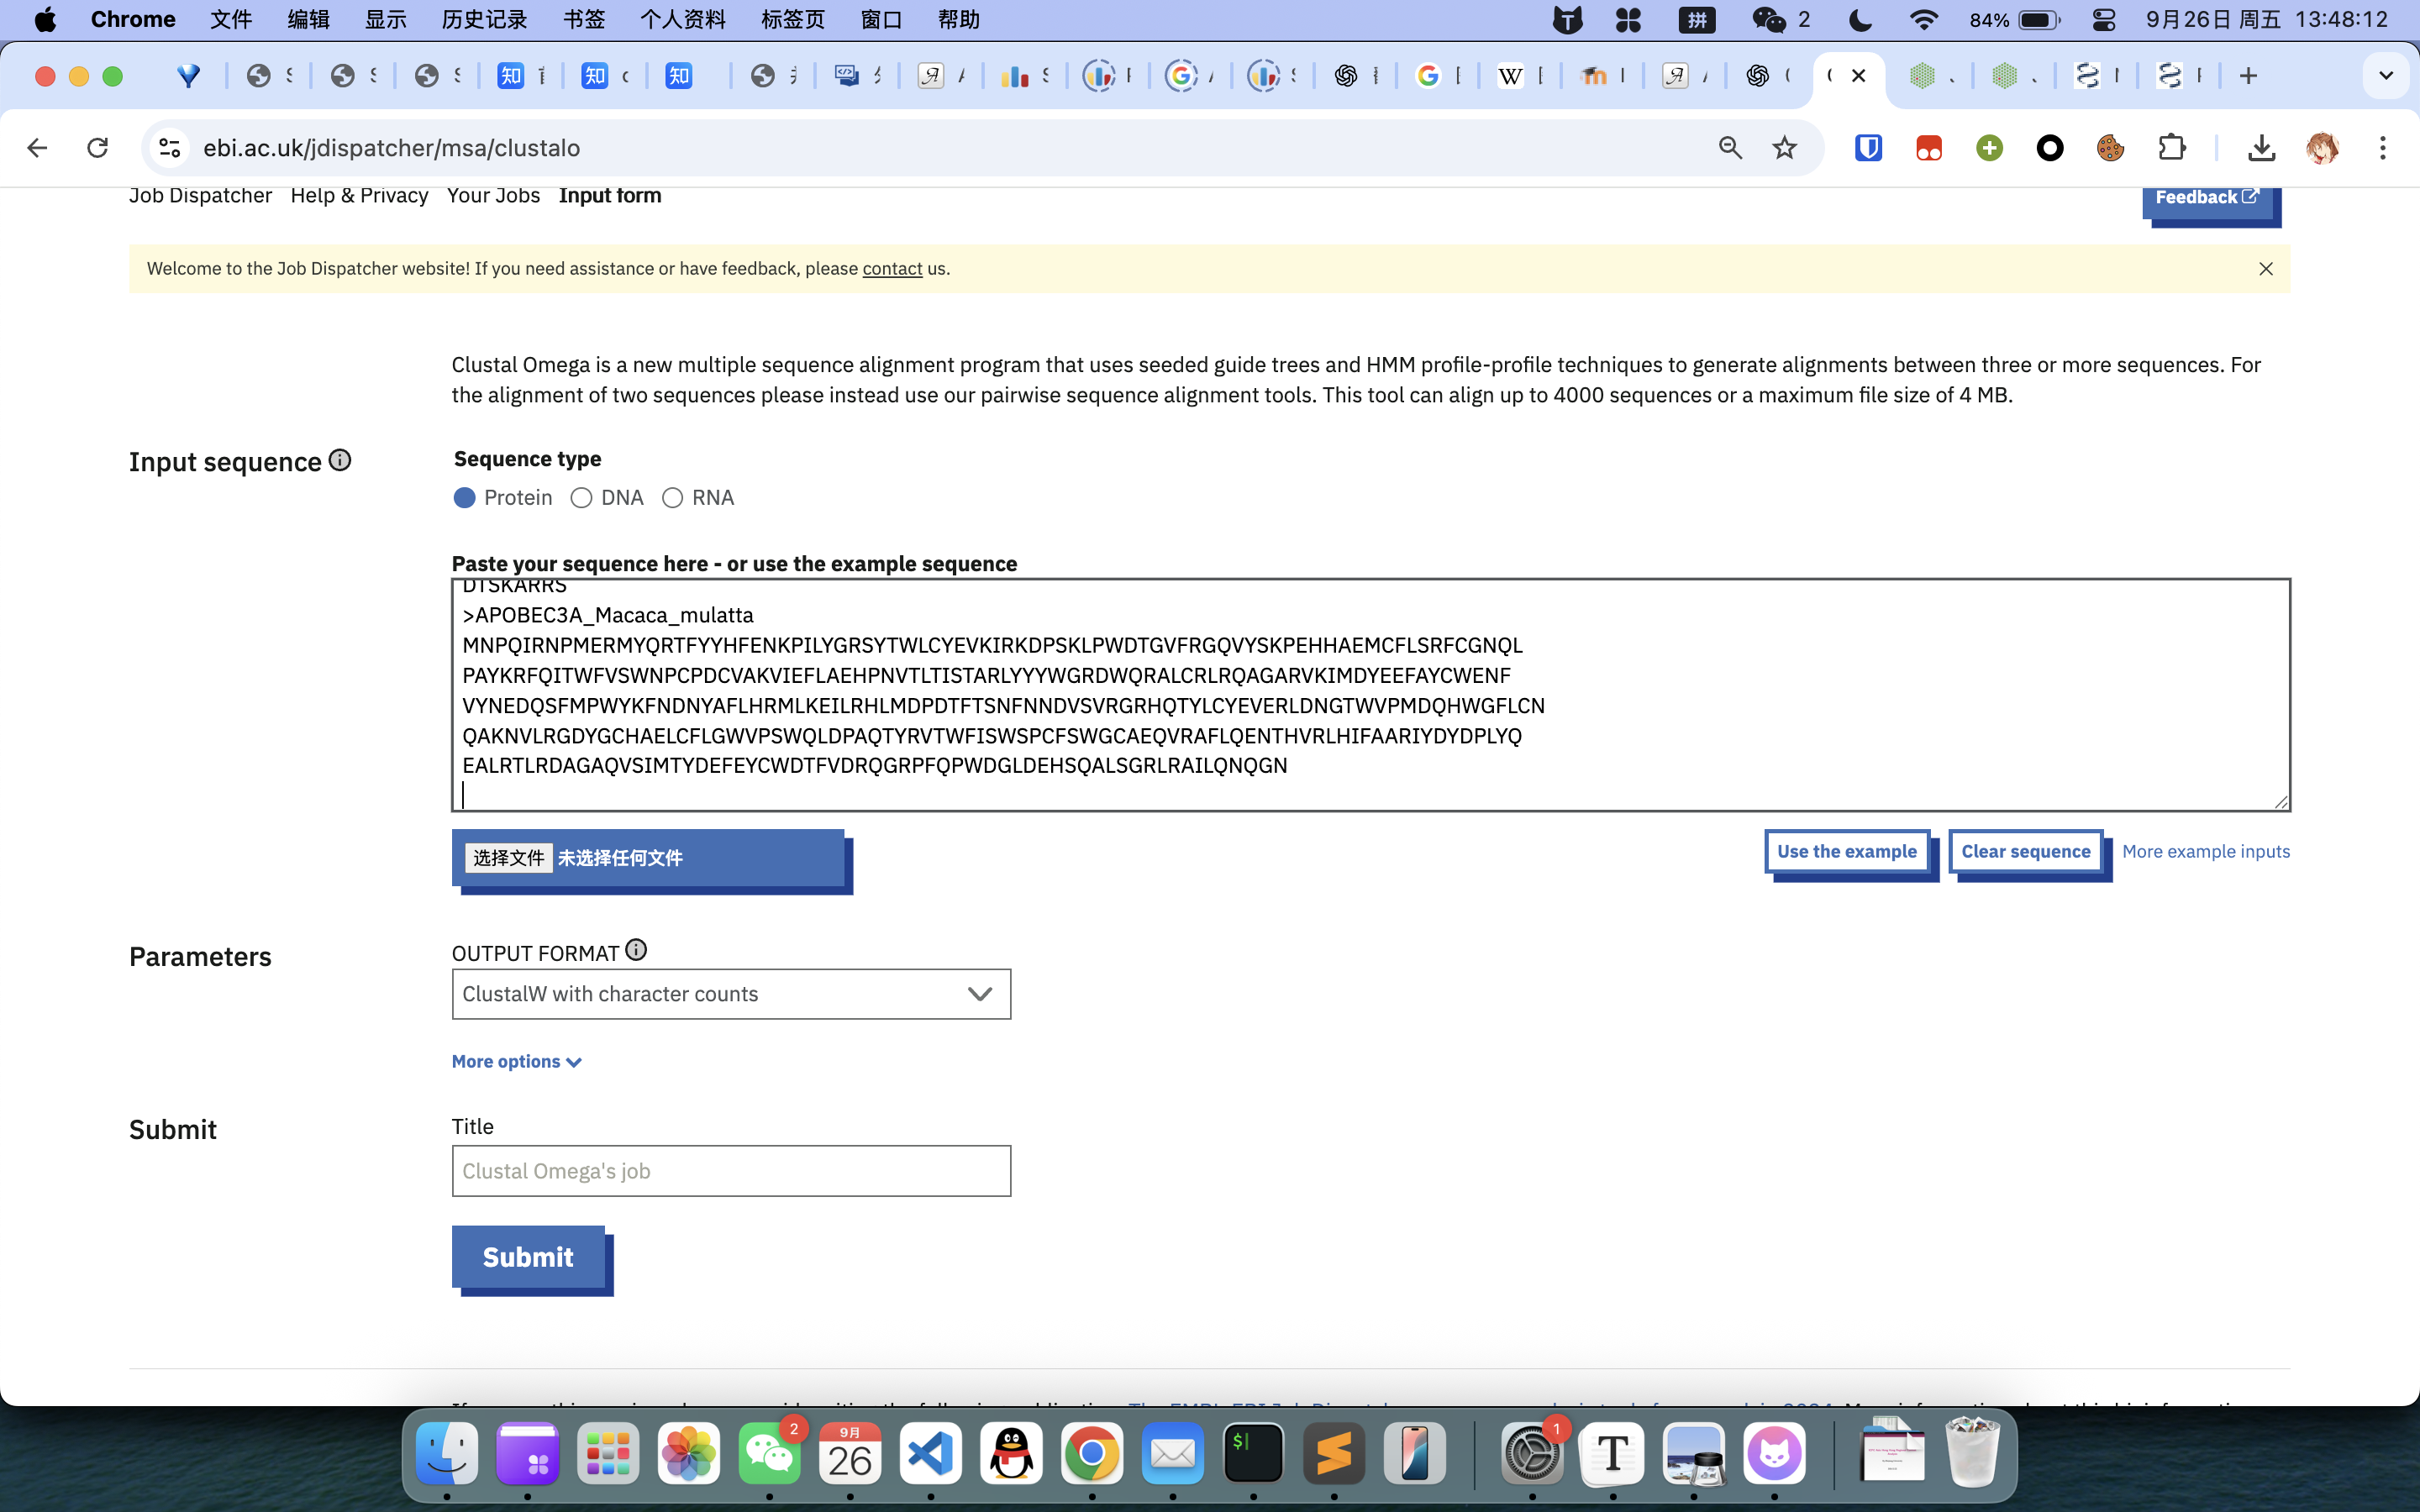
\includegraphics[width=1\textwidth]{../images/task2/image1.png}
\end{center}
\begin{center}
    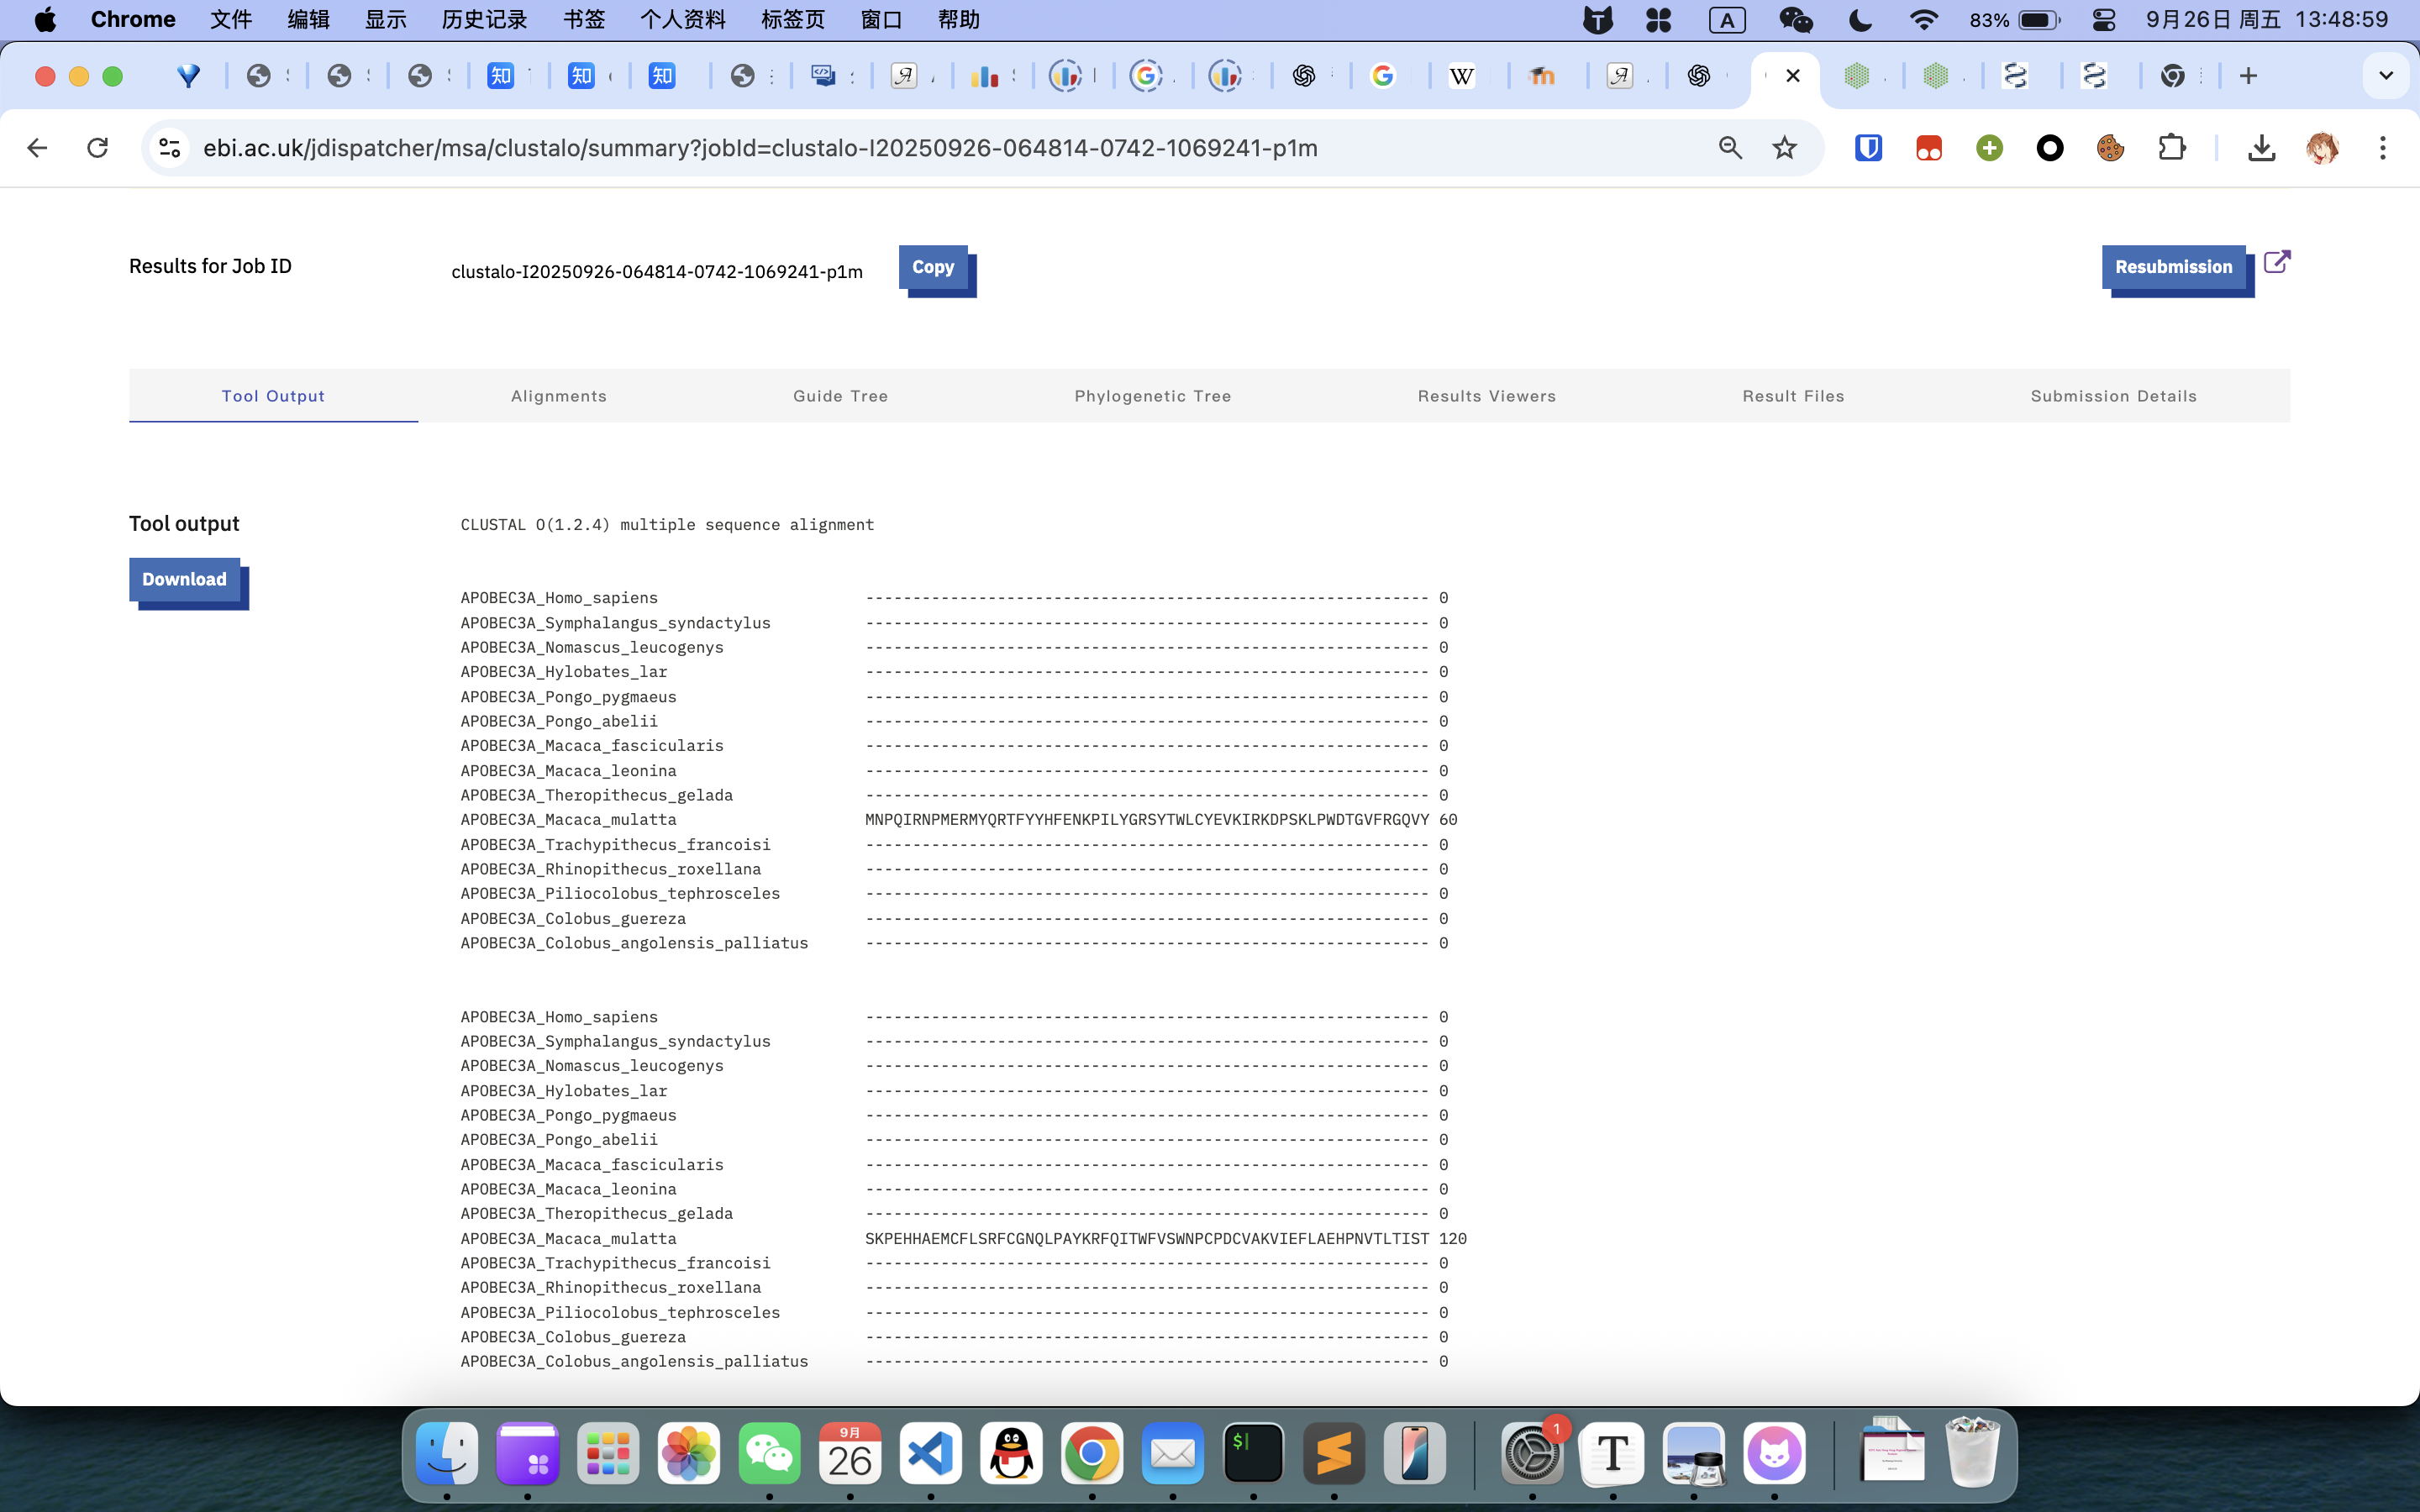
\includegraphics[width=1\textwidth]{../images/task2/image2.png}
\end{center}
\begin{center}
    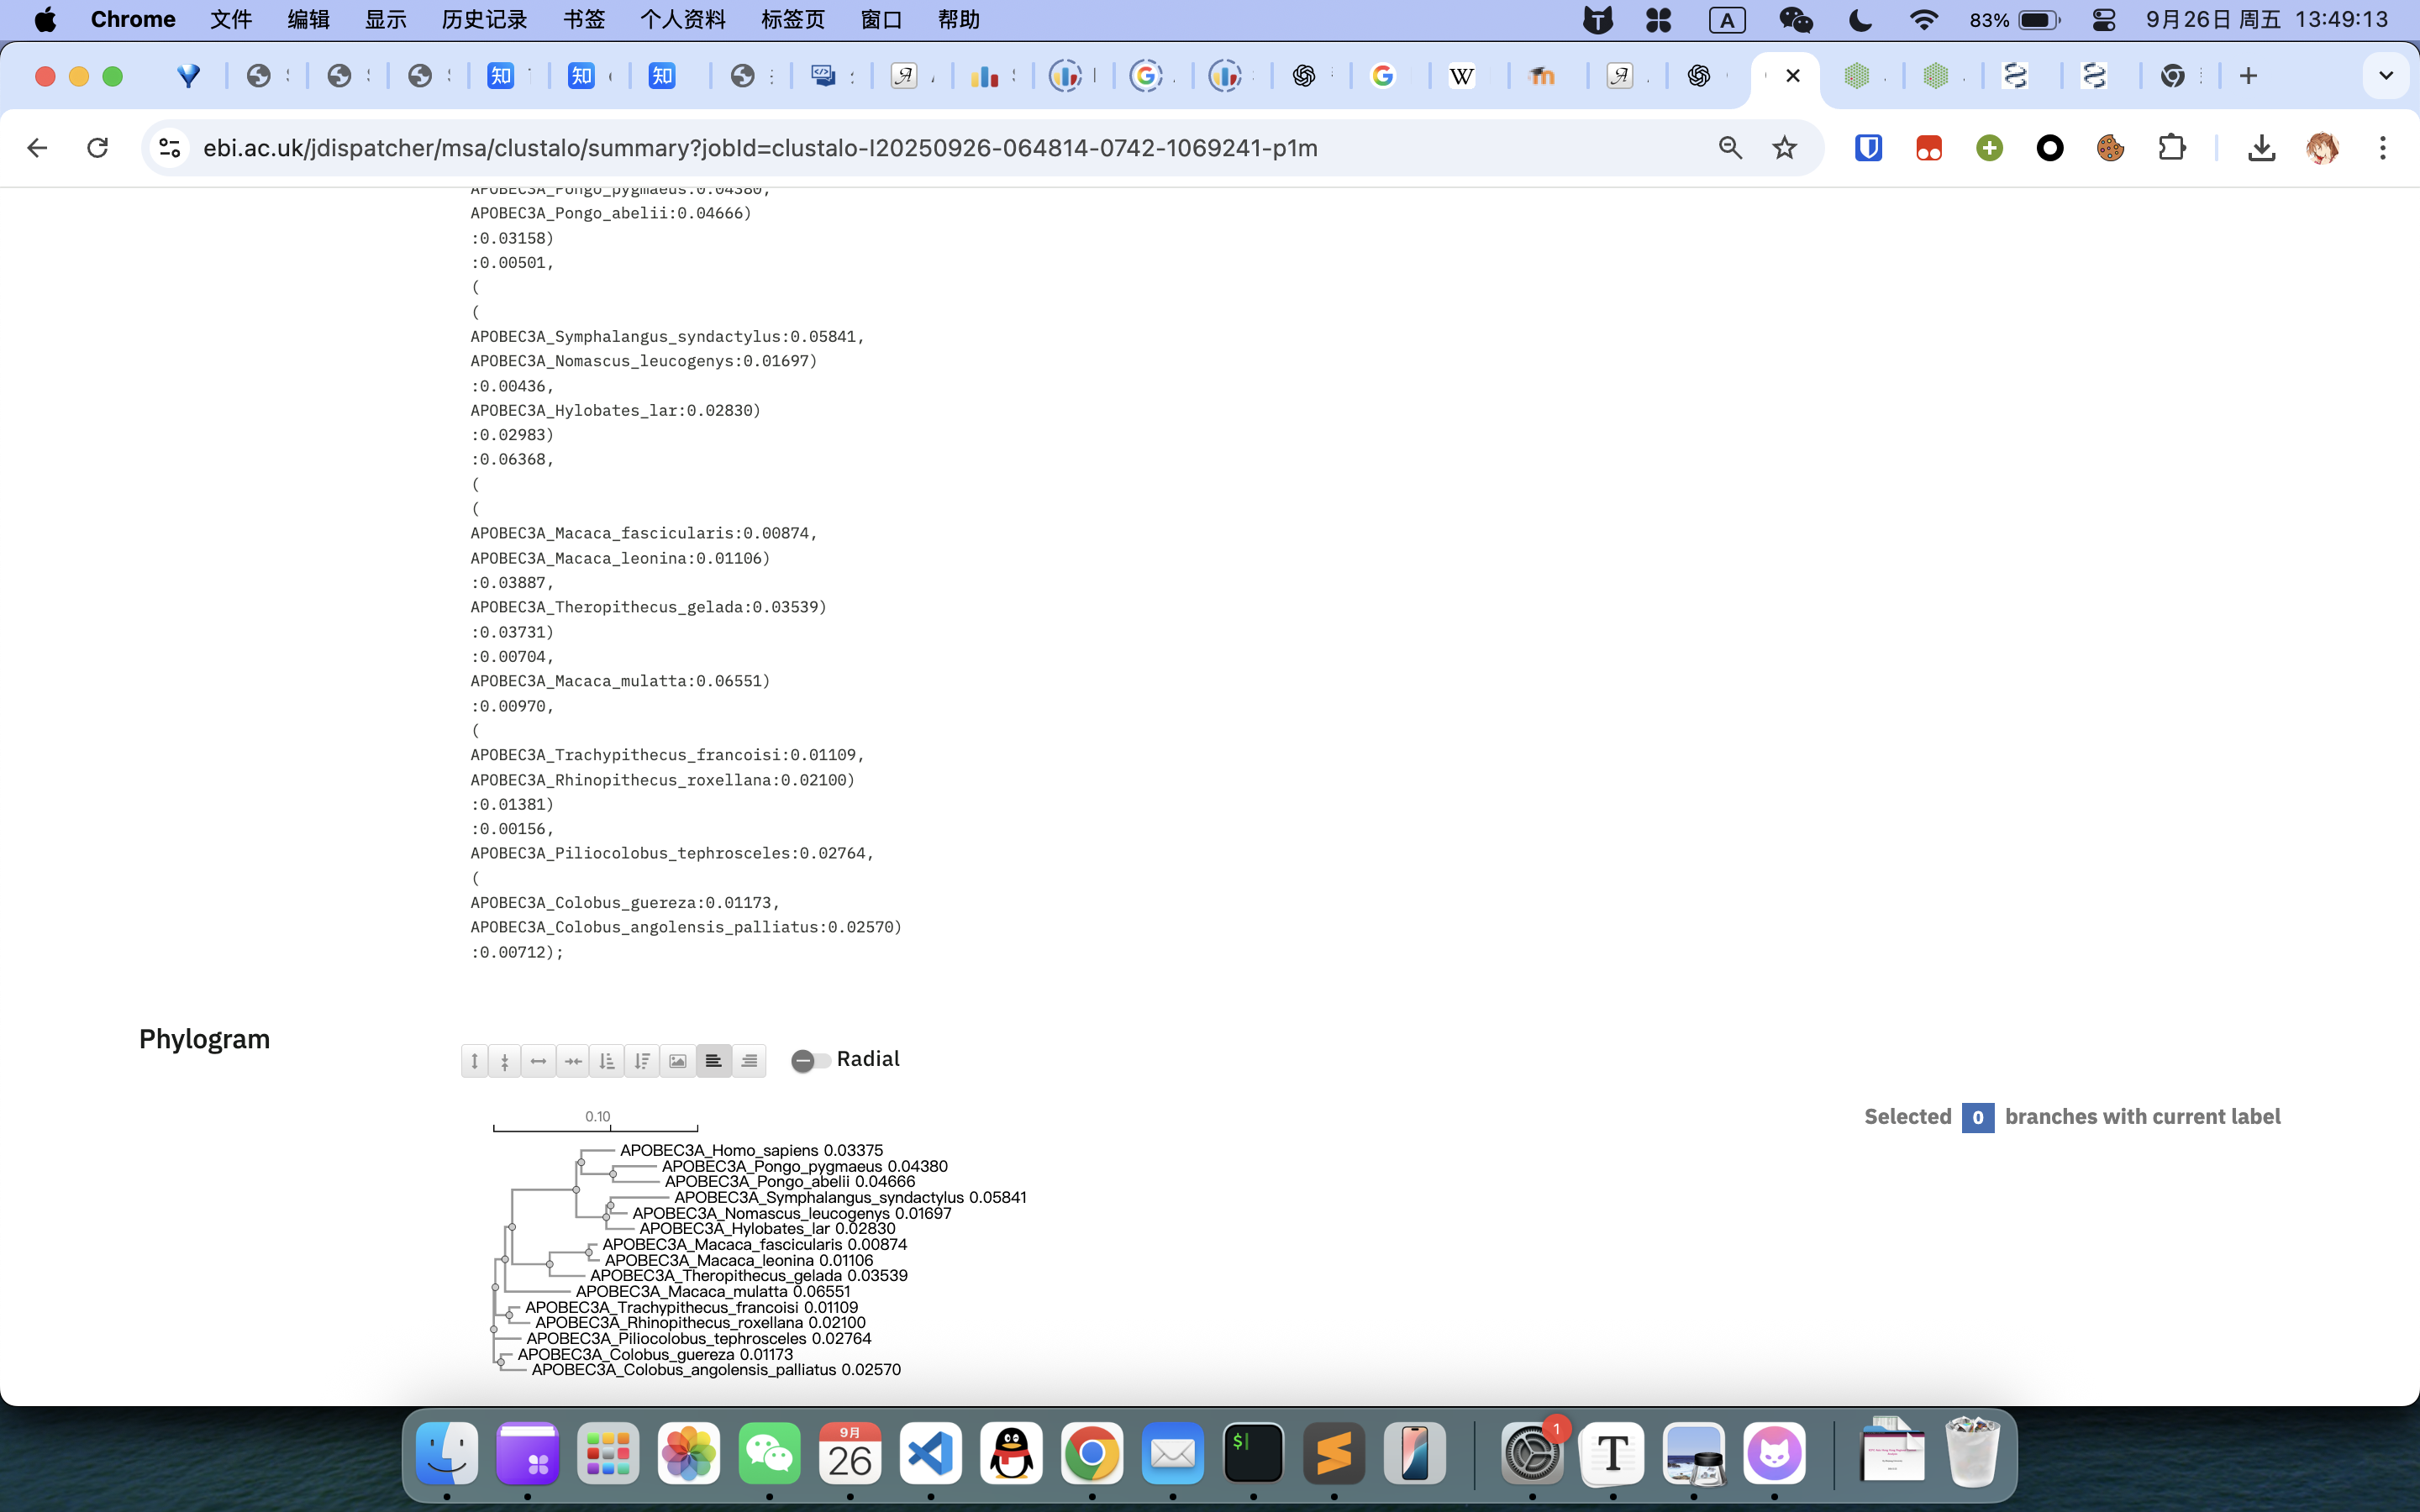
\includegraphics[width=1\textwidth]{../images/task2/image3.png}
\end{center}

\section{Task 3}

\begin{center}
    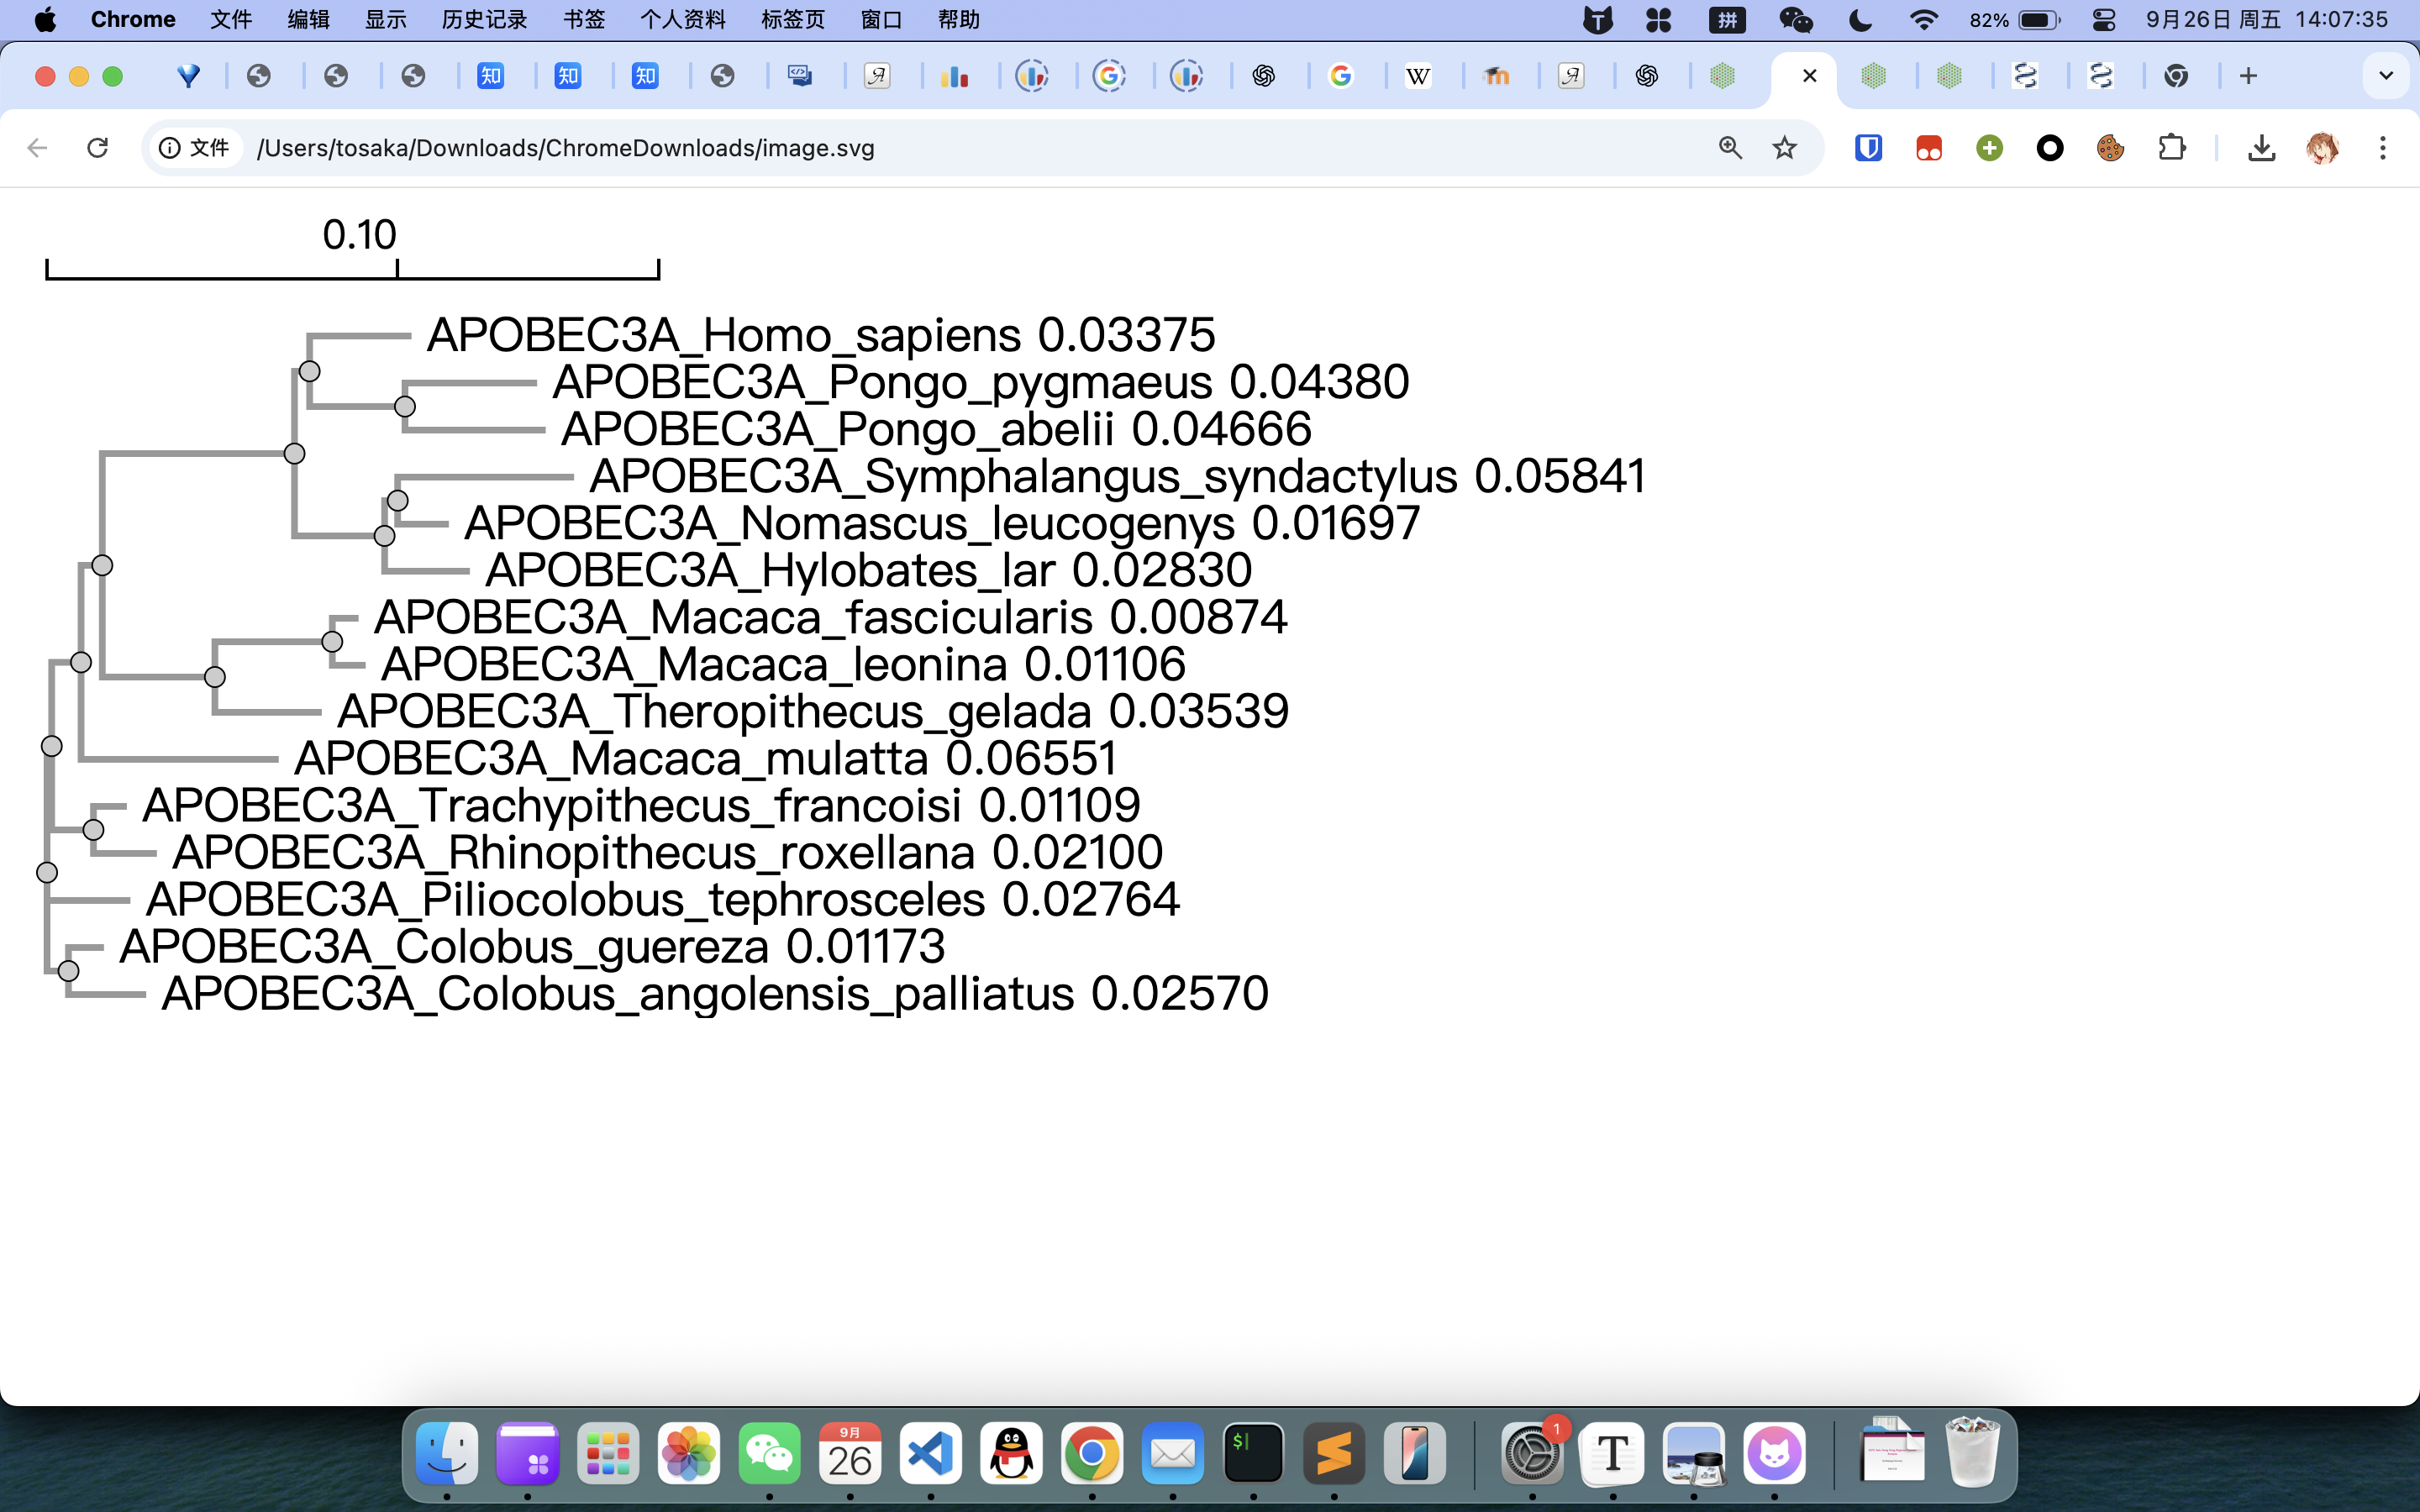
\includegraphics[width=1\textwidth]{../images/task3/image1.png}
\end{center}

The tree demonstrates that \textit{Homo sapiens} clusters most closely with \textit{Pongo pygmaeus} (Bornean orangutan) and \textit{Pongo abelii} (Sumatran orangutan), indicating a very close evolutionary relationship.

The phylogenetic tree aligns perfectly with the established evolutionary relationships among primates. The close grouping of humans (\textit{Homo sapiens}) with orangutans (\textit{Pongo}) reflects their shared ancestry as hominids. The more distant relationships with gibbons, macaques, and colobus monkeys are also consistent with known primate phylogeny.

This indicates that the APOBEC3A gene has evolved in a manner that mirrors the speciation events of its host organisms.

\section{Task 4}

\begin{center}
    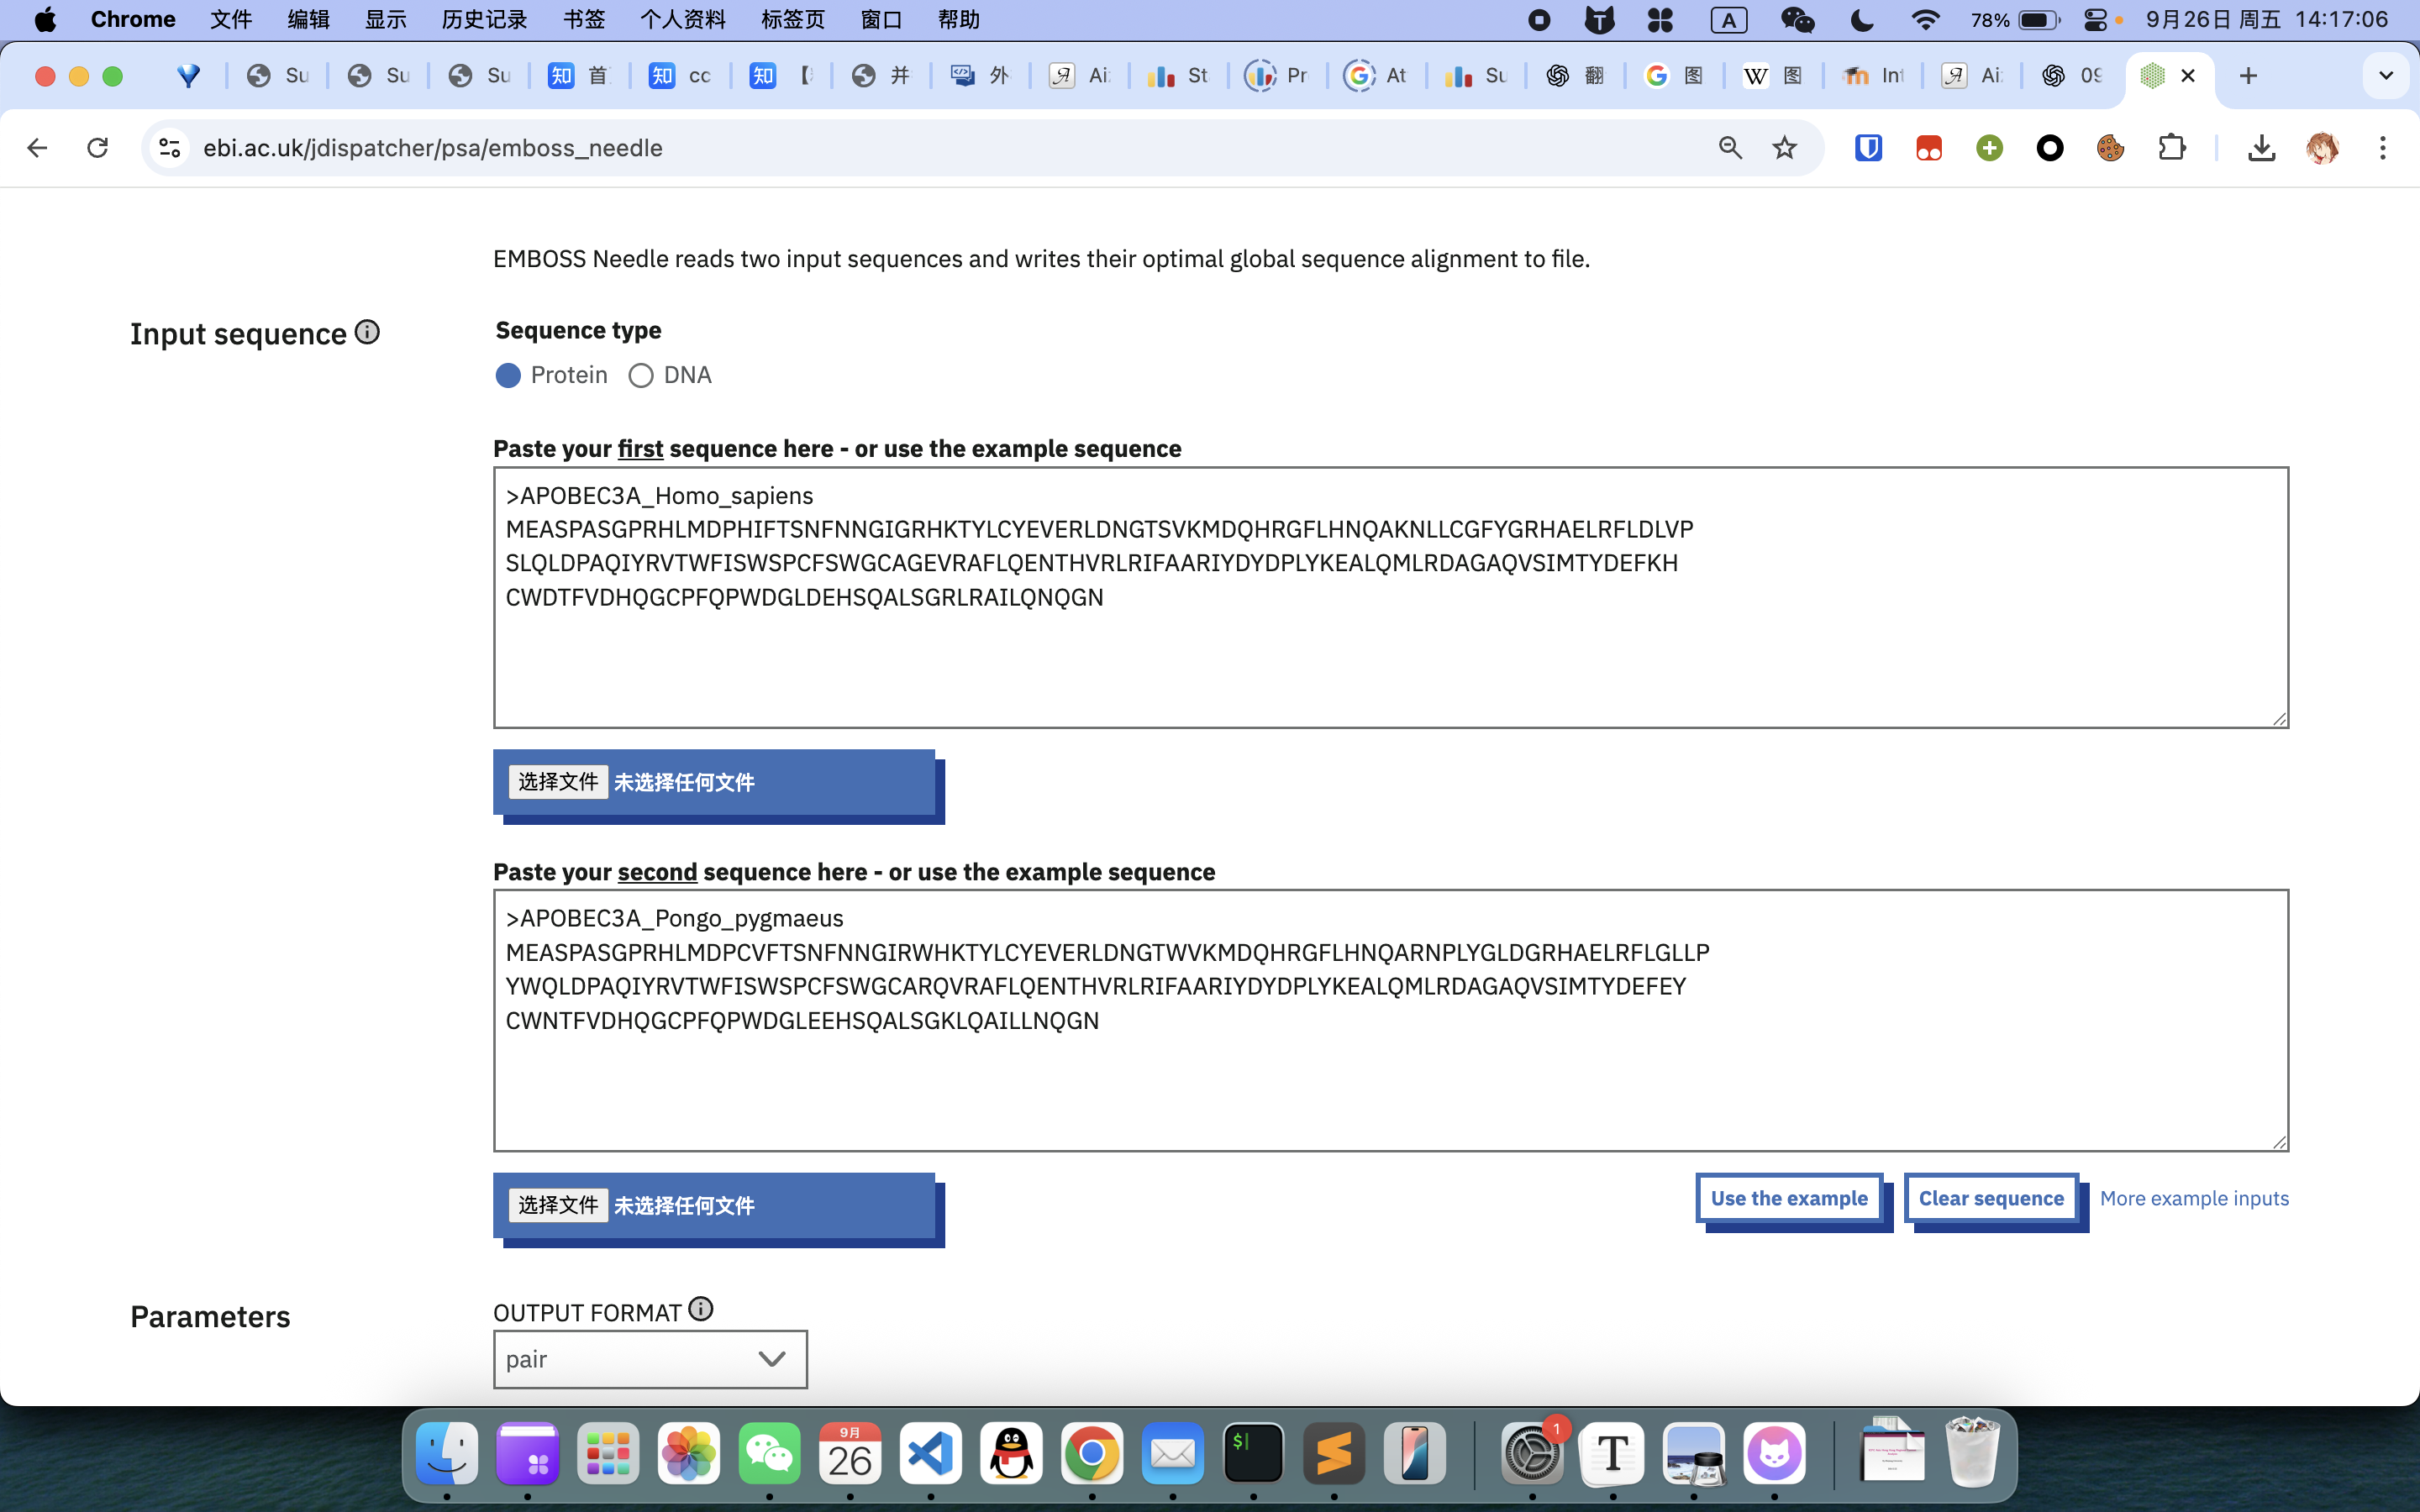
\includegraphics[width=1\textwidth]{../images/task4/image1.png}
\end{center}
\begin{center}
    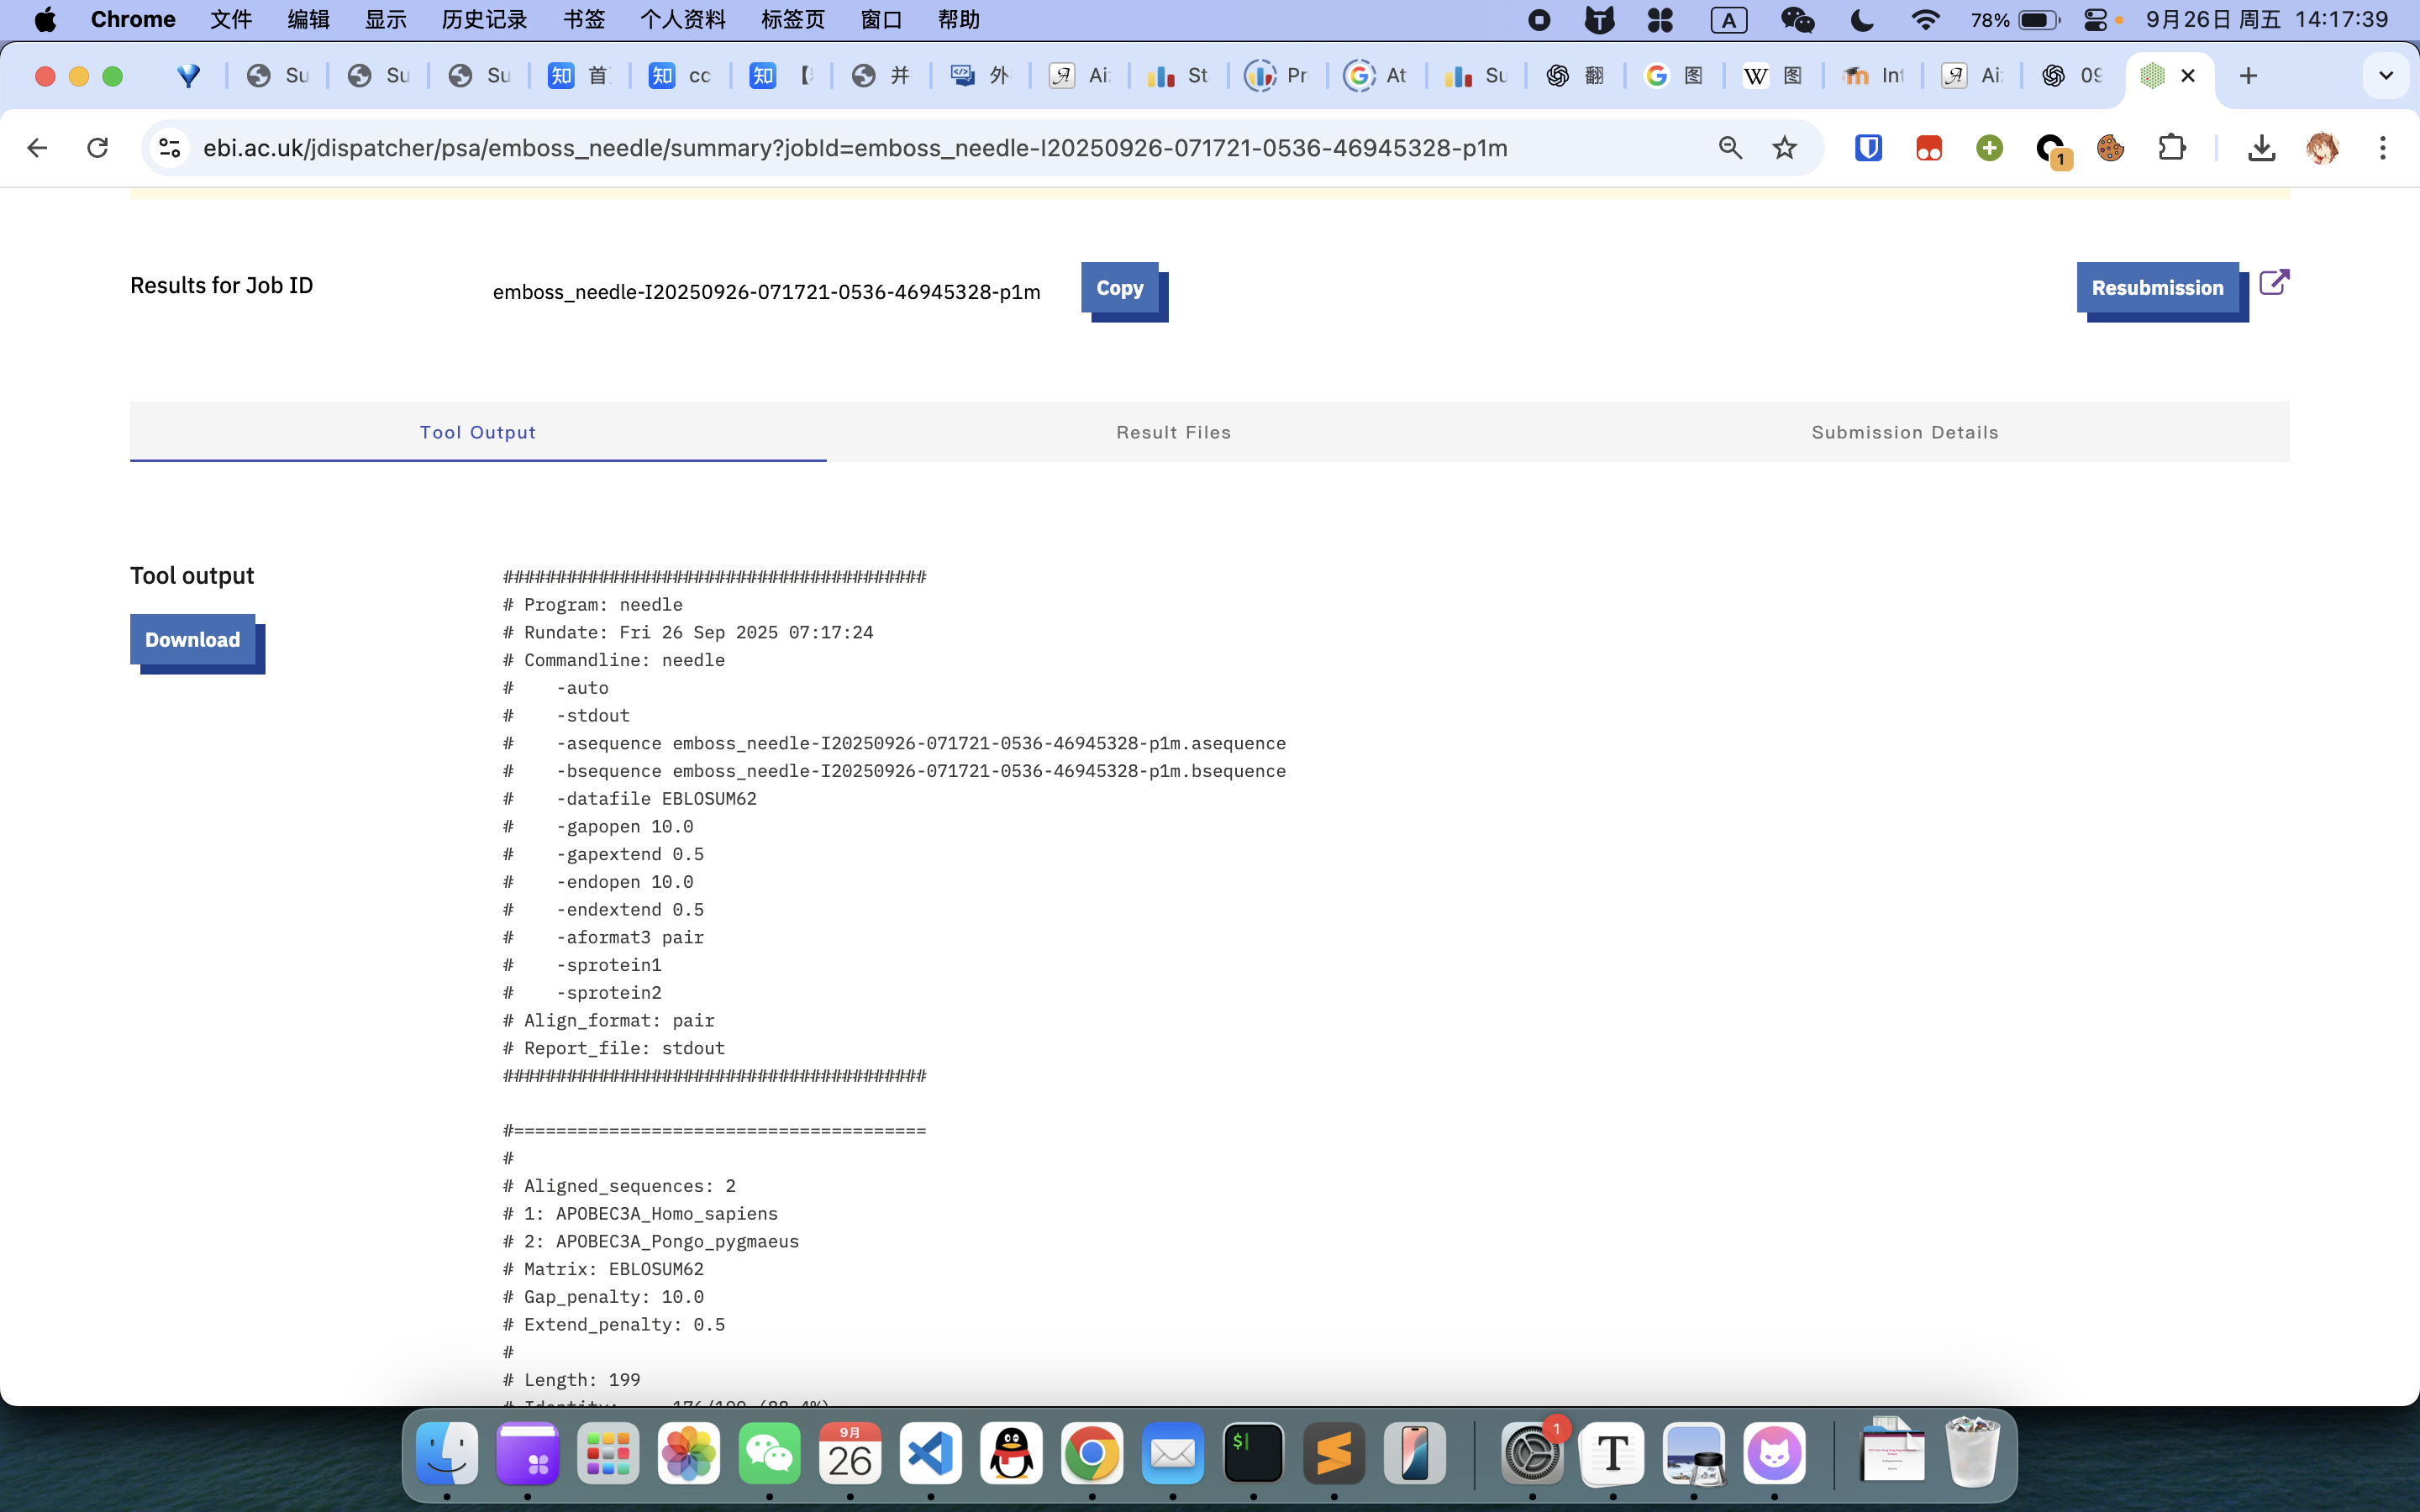
\includegraphics[width=1\textwidth]{../images/task4/image2.png}
\end{center}

The pairwise alignment of APOBEC3A from \textit{Homo sapiens} and \textit{Pongo pygmaeus} yielded the following summary statistics:

\begin{itemize}
    \item \textbf{Length:} 199 amino acids
    \item \textbf{Identity:} 176/199 (88.4\%)
    \item \textbf{Similarity:} 186/199 (93.5\%)
    \item \textbf{Gaps:} 0/199 (0.0\%)
    \item \textbf{Score:} 962.0
\end{itemize}

The detailed alignment output is presented in Listing \ref{lst:alignment}.

\begin{lstlisting}[language=bash, caption={EMBOSS Needle Alignment Output}, label={lst:alignment}]
#=======================================
# Aligned_sequences: 2
# 1: APOBEC3A_Homo_sapiens
# 2: APOBEC3A_Pongo_pygmaeus
# Matrix: EBLOSUM62
# Length: 199
# Identity:     176/199 (88.4%)
# Similarity:   186/199 (93.5%)
# Gaps:           0/199 ( 0.0%)
# Score: 962.0
#=======================================

APOBEC3A_Homo      1 MEASPASGPRHLMDPHIFTSNFNNGIGRHKTYLCYEVERLDNGTSVKMDQ     50
                     |||||||||||||||.:|||||||||..||||||||||||||||.|||||
APOBEC3A_Pong      1 MEASPASGPRHLMDPCVFTSNFNNGIRWHKTYLCYEVERLDNGTWVKMDQ     50

APOBEC3A_Homo     51 HRGFLHNQAKNLLCGFYGRHAELRFLDLVPSLQLDPAQIYRVTWFISWSP    100
                     |||||||||:|.|.|..|||||||||.|:|..||||||||||||||||||
APOBEC3A_Pong     51 HRGFLHNQARNPLYGLDGRHAELRFLGLLPYWQLDPAQIYRVTWFISWSP    100

APOBEC3A_Homo    101 CFSWGCAGEVRAFLQENTHVRLRIFAARIYDYDPLYKEALQMLRDAGAQV    150
                     |||||||.:|||||||||||||||||||||||||||||||||||||||||
APOBEC3A_Pong    101 CFSWGCARQVRAFLQENTHVRLRIFAARIYDYDPLYKEALQMLRDAGAQV    150

APOBEC3A_Homo    151 SIMTYDEFKHCWDTFVDHQGCPFQPWDGLDEHSQALSGRLRAILQNQGN    199
                     ||||||||::||:||||||||||||||||:||||||||:|:|||.||||
APOBEC3A_Pong    151 SIMTYDEFEYCWNTFVDHQGCPFQPWDGLEEHSQALSGKLQAILLNQGN    199
\end{lstlisting}

\paragraph{Specific Amino Acid Differences:}
Despite the overall similarity, 23 amino acid positions differ between the two sequences. Some notable substitutions include:
\begin{itemize}
    \item \textbf{Position 15:} Histidine (H) in humans is replaced by Cysteine (C) in orangutans.
    \item \textbf{Position 61-64:} The `KNLL` motif in humans corresponds to `RNPL` in orangutans, showing a cluster of substitutions in this region.
    \item \textbf{Position 158-159:} The `HC` (Histidine-Cysteine) motif in humans is substituted by `EY` (Glutamic acid-Tyrosine) in orangutans, representing two consecutive changes to residues with different biochemical properties.
\end{itemize}
It is important to note that many substitutions are conservative (e.g., Arginine `R` to Lysine `K` at position 179), where the replacing amino acid shares similar properties (in this case, both are basic and positively charged). Such changes are less likely to disrupt protein structure and function.

\end{document}
